\section{\ms}
\label{sec:method}

A design is one Python file exposing a \code{build(p)} function decorated with \code{@design},
which declares typed parameters with ranges and named poses. It returns a \code{Robot}. All units
are millimetres and radians in one world frame at the home pose (x forward, y left, z up).
\Cref{fig:gallery} shows the bundled designs.

\begin{figure*}[t]
  \centering
  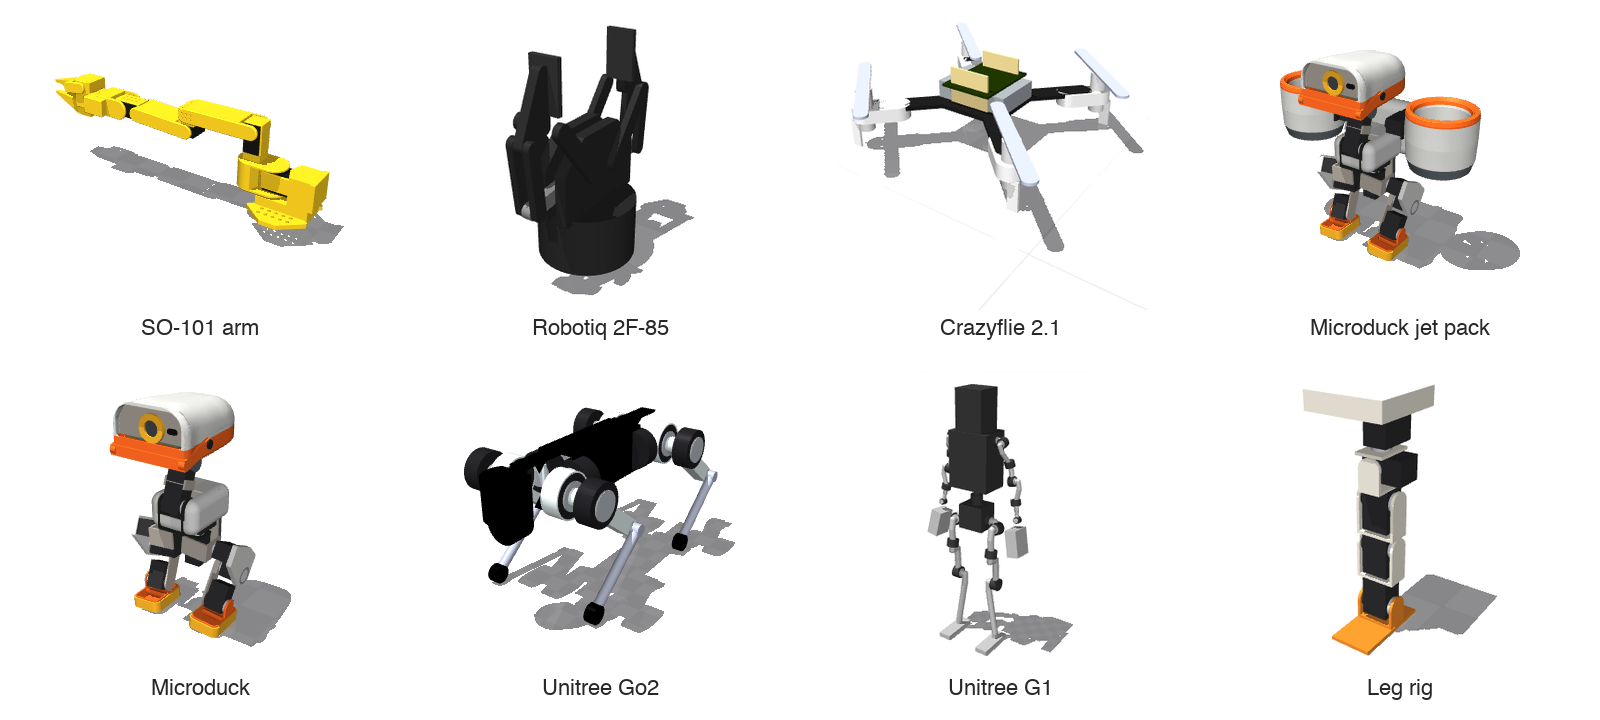
\includegraphics[width=\textwidth]{gallery.png}
  \caption{The bundled designs as built by \ms. Six are rebuilt from public reference models,
  without using the references' meshes; the jet-pack Microduck and the single leg are new designs.}
  \label{fig:gallery}
\end{figure*}

\subsection{Connections}
\label{sec:connect}
A \emph{connector} is a frame on a part's surface whose $z$ axis is the outward normal and $x$ the
reference direction. Its position is checked to lie on the part's surface when it is declared.
Parts are placed only by connection, root outward:
\begin{itemize}
\item \code{fasten(a, b, spin, at)} places $b$ so that its connector faces $a$'s, with
  normals opposed; \code{spin} fixes the free rotation about the normal and \code{at} slides
  the contact along $a$'s face (checked to stay on it).
\item \code{attach(base, part)} admits a shape drawn in world coordinates (a shell, a cover) only
  if it touches \code{base}; otherwise it raises an error reporting the gap.
\item \code{joint(name, actuator, range)} makes a placed servo or motor the joint between its
  case and its output; \code{hinge} adds an unactuated pin whose axis must pass through both
  parts, and a hinge between parts already connected closes a kinematic loop.
\item Higher-level constructors are built from these: \code{link} draws a printed link around a
  servo, cut clear of its swept volume and pocketed for the next one; \code{chain} builds a limb
  from a joint table; \code{rotor} adds thrust and reaction torque.
\end{itemize}
Because placement is computed and contact is checked at each call, the robot is a connected graph
of touching parts by construction. Re-connecting an already placed part must agree with its pose,
which catches over-constrained mistakes.
\note{Add a formal statement: invariant (every part reachable from the root through checked
contacts) and the proof sketch by induction over calls.}

\subsection{Derivation}
\label{sec:derive}
\code{robot()} contracts rigidly connected parts into links and splits them at joints, giving the
kinematic tree. Joint anchors and axes come from the actuator frames; inertias from the solids at a
material density and, for printed parts, an infill model fitted to measured masses; actuator gains,
armature and limits from datasheets (armature $=$ rotor inertia $\times$ (gear ratio)$^2$).
\code{mirror} with prefixes \code{left\_} and \code{right\_} produces the other side under an explicit axis convention,
since vendors differ in whether mirrored joints keep or flip their axes.

\subsection{The build report}
\label{sec:report}
A build writes MJCF, URDF, an MJX variant with primitive collisions, renders and a JSON report:
\begin{itemize}
\item \textbf{Mass} per body and total.
\item \textbf{Interference}: overlapping part pairs at home, and for every joint a sweep over its
  declared range reporting the usable interval and the first colliding pair at each end.
\item \textbf{Class test}: floating-base robots must hold \code{home} for 3\,s on actuator PD alone
  (reporting settled pitch, the weakest actuator and a stiffness ratio); rotorcraft are trimmed,
  disturbed by $10^\circ$ and must recover in closed loop; fixed-base arms report actuator load at
  full reach with a payload.
\end{itemize}
Every parameter override is validated against its declared range before building.
\note{Figure 2: one design snippet, the AttachmentError it raises when a number is wrong, and the
report fragment after the fix. Source: README example.}
